\documentclass[10pt]{report}
\usepackage[utf8]{inputenc}
\usepackage[danish]{babel}
\usepackage [T1]{fontenc}
\usepackage[margin=2.5cm, headheight=36pt]{geometry}
\usepackage[hidelinks]{hyperref}
\usepackage{graphicx}
\graphicspath{{figures/}{Billeder/}}
\usepackage{listings}
\usepackage{color}
\usepackage{adjustbox}
\usepackage{tocloft}
\usepackage{listings}
\usepackage{enumitem}
\usepackage{indentfirst}
\usepackage{caption}
\usepackage{float}
\usepackage{lmodern,textcomp}
\usepackage{varwidth}
\usepackage{amsmath}

\usepackage{fourier}
\usepackage{array}
\usepackage{makecell}
\renewcommand\theadalign{bc}
\renewcommand\theadfont{\bfseries}
\renewcommand\theadgape{\Gape[3.5pt]}
\renewcommand\cellgape{\Gape[3.5pt]}


\usepackage{fancyhdr}
\fancypagestyle{fancy}{
  \fancyhf{} % clear all header and footer fields
  \fancyhead[L]{av105 - Andreas Vikke\\mf237 - Martin Frederiksen}
  \fancyhead[R]{\today\\}
  \fancyfoot[R]{Side \thepage}
  \renewcommand{\headrulewidth}{0.4pt}% Line at the header visible
  \renewcommand{\footrulewidth}{0.4pt}% Line at the footer visible
}
\fancypagestyle{plain}{%
  \fancyhf{} % clear all header and footer fields
  \fancyhead[L]{av105 - Andreas Vikke\\mf237 - Martin Frederiksen}
  \fancyhead[R]{\today\\}
  \fancyfoot[R]{Side \thepage}
  \renewcommand{\headrulewidth}{0.4pt}% Line at the header visible
  \renewcommand{\footrulewidth}{0.4pt}% Line at the footer visible
}

\renewcommand\thefootnote{\textcolor{black}{\arabic{footnote}}}

\hypersetup{
colorlinks=true,
linkcolor=black,
citecolor=green,
filecolor=magenta,
urlcolor=cyan
}

\setlength{\parskip}{6pt}

\definecolor{dkgreen}{rgb}{0,0.6,0}
\definecolor{gray}{rgb}{0.5,0.5,0.5}
\definecolor{mauve}{rgb}{0.58,0,0.82}
\definecolor{bluekeywords}{rgb}{0.13,0.13,1}
\definecolor{greencomments}{rgb}{0,0.5,0}
\definecolor{turqusnumbers}{rgb}{0.17,0.57,0.69}
\definecolor{redstrings}{rgb}{0.5,0,0}

\lstset{frame=tb,
  language=Java,
  aboveskip=3mm,
  belowskip=3mm,
  showstringspaces=false,
  columns=flexible,
  basicstyle={\small\ttfamily},
  numbers=none,
  numberstyle=\tiny\color{gray},
  keywordstyle=\color{blue},
  commentstyle=\color{dkgreen},
  stringstyle=\color{mauve},
  breaklines=true,
  breakatwhitespace=true,
  tabsize=3
}

\lstdefinelanguage{FSharp}
                {morekeywords={let, new, match, with, rec, open, module, namespace, type, of, member, and, for, in, do, begin, end, fun, function, try, mutable, if, then, else},
    keywordstyle=\color{bluekeywords},
    sensitive=false,
    morecomment=[l][\color{greencomments}]{///},
    morecomment=[l][\color{greencomments}]{//},
    morecomment=[s][\color{greencomments}]{{(*}{*)}},
    morestring=[b]",
    stringstyle=\color{redstrings}
    }


\date{}

\begin{document}
\begin{titlepage}
  \begin{center}
    \vspace*{1cm}

    \Huge
    \textbf{Homework Assignment}
         
    \vspace{1.5cm}

    \LARGE
    \textbf{Andreas Vikke \& Martin Frederiksen}

    \vfill
  
    
\includegraphics[width=0.4\textwidth]{7fe3c3f6-Stego}
    
    \vfill
    
    \Large
    \today\\
    Professionsbachelor i softwareudvikling\\
    Cphbusiness Lyngby\\
    Denmark
         
  \end{center}
\end{titlepage}

\chapter*{1. Description}
\addcontentsline{toc}{chapter}{1.  Description}
\pagestyle{fancy}
\noindent In order to look at self reflection and to judge your assessment of information, you should solve the programming exercise below.

\noindent However - the important thing in this exercise is how you solved it, not the end result.

\noindent At the end of the programming exercise you should have:

\begin{itemize}
  \item A list of \textbf{all} search queries you made to solve it, and timestamps (just copy it from the browser history)
  \item A list all pages you visited to solve it (just copy it from the browser history)
  \item A list of the 3 biggest stumbling blocks you came across and your reflection on why they were problematic (did you misunderstand something, was some of the info you found wrong, did you miss a detail, …)
  \item A brief "every 30 min" diary as explained in the slides (this is more frequent than one would normally do, and is just meant as part of the exercise)
\end{itemize}

\chapter*{2. Løsning}
\addcontentsline{toc}{chapter}{2. Løsning}
\pagestyle{fancy}
\noindent Vi valgte at bruge Python som programmingssprog og vi har bygget det som en docker container. Nedenfor ses en række billeder af hvordan projektet kan køres, samt vores løsnings forslag med tilhørende resultat.

\begin{figure}[H]
  \centering
  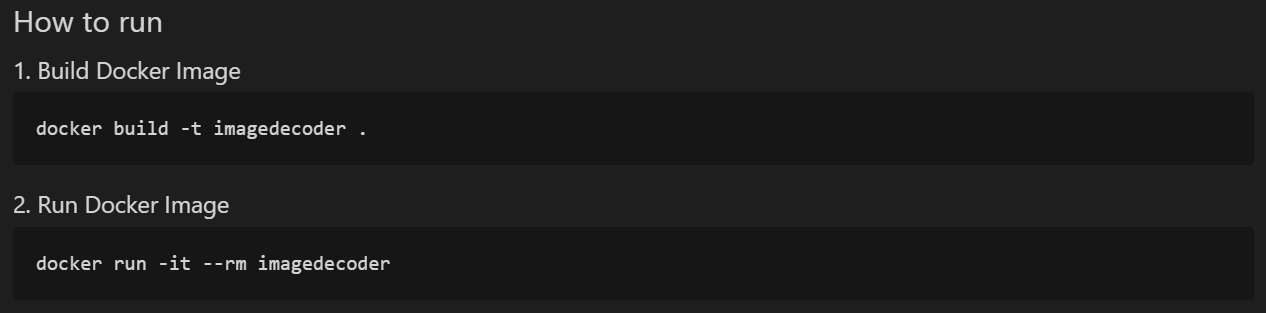
\includegraphics[width=\textwidth]{HowToRun.png}
  \caption{Billede af kommandoer der kan bruges til at køre projektet.}
\end{figure}

\begin{figure}[H]
  \centering
  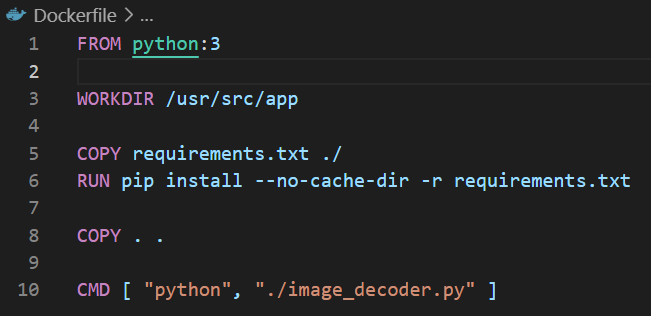
\includegraphics[width=\textwidth]{Dockerfile.png}
  \caption{Billede af vores dockerfil.}
\end{figure}

\begin{figure}[H]
  \centering
  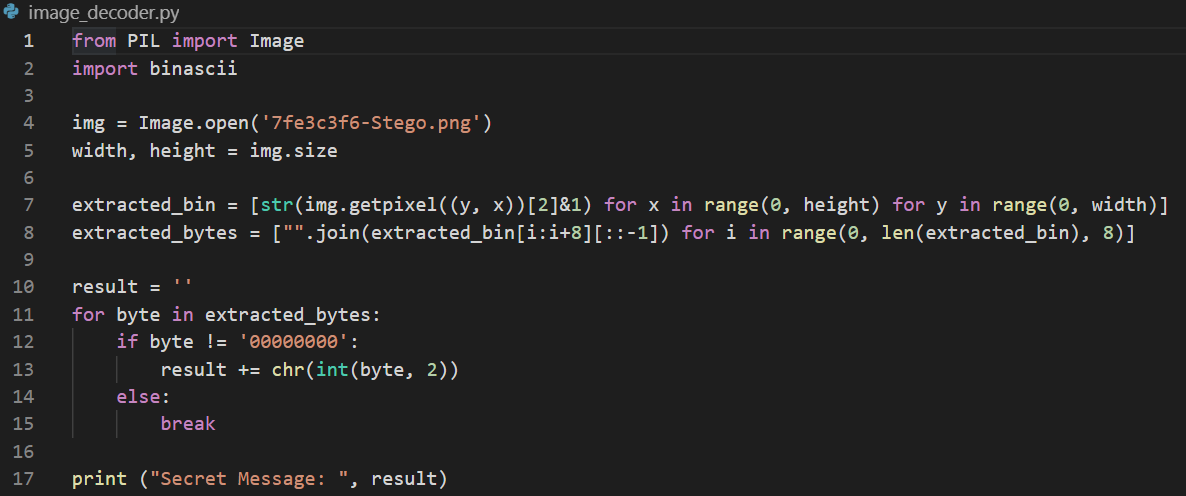
\includegraphics[width=\textwidth]{Pythonkode.png}
  \caption{Billede af vores pythonkode.}
\end{figure}

\begin{figure}[H]
  \centering
  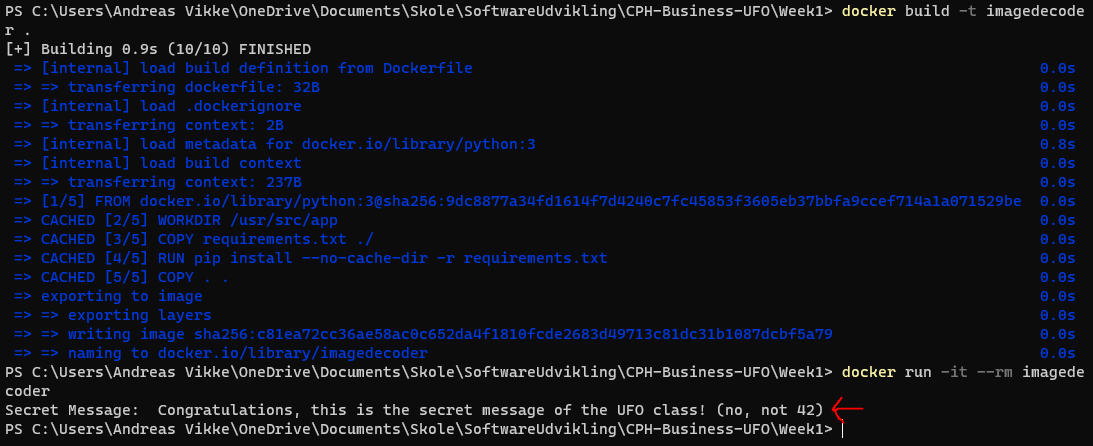
\includegraphics[width=\textwidth]{Result.png}
  \caption{Billede af resultatet.}
\end{figure}

\chapter*{3. Største udfordringer}
\addcontentsline{toc}{chapter}{3. Største udfordringer}
\pagestyle{fancy}
\begin{itemize}
  \item \textbf{Forståelse af opgaven:} det største problem for vores gruppe var at forstå opgaven. Vi prøvede hver især først at decode billedet uden noget meningsfuldt resultat. Vi brugte dernæst lidt tid på lige at få snakket opgaven ordenligt igennem sådan at der ikke var nogen tvivl om hvad der præsist skulle ske. Altså den klassike programmørfejl med at starte på opgaven før den overhovedet er forstået.
  \item \textbf{Least significant bit of the blue values:} dette brugte vi lidt tid på at forstå ordenligt i forhold til at vi skal tage det sidste bit i den blå del af pixlen. Hvis vi printede en pixel ud fik vi RGBA værdien ud som (R, G, B, A) hvor A er alpha og beskriver transparens i den givne pixel. Derudover stod det ikke 100\% klart at \textit{Least significant} betød den sidste bit i farve værdien.
  \item \textbf{Little-endian:} her var vi langsomme om at opfatte at hver byte var spejlvendt.
\end{itemize}

\chapter*{4. Dagbog}
\addcontentsline{toc}{chapter}{4. Dagbog}
\pagestyle{fancy}

\noindent\textbf{05/01-21 kl. 14.07:}\\
\noindent Da vi hver især bare kastede os ud i opgaven uden held brugte vi tiden på det første møde til at gennemgå opgaven samlet. På den måde kunne alle parter blive enige om hvad der præsist skulle ske. Vores gruppe havde hver især også problemer med at forstå enkelte ord/begreber i opgaven og under mødet kunne vi svare hinanden på hvad ordene/begreberne betød.

\noindent\textbf{05/01-21 kl. 14.45:}\\
\noindent Efter vi havde fået en forståelse af opgaven kunne vi begynde at arbejde rigtig på en løsning. Vi løb så ind i det næste problem før dette møde, hvilket var at forstå det output ordenligt som vi fik da vi så på en bestemet pixel. Vi var lidt i tvivl om hvad den sidst bit betød i forhold til pxilen da vi så på 4 værdier og ikke kun 3. Vi undersøgte så dette under mødet og kunne derved konstatere at den sidste værdi i pixlen er den værdi der beskriver hvor transparent pixlen er. Derudover var vi nødt til igen at undersøge hvad \textit{Least significant} betød eftersom vi ikke havde den rette forståelse da det kom til stykket.

\noindent\textbf{05/01-21 kl. 15.20:}\\
\noinden Under dette møde havde vi en følelse af at vi var ved at være i mål. Vi havde nu alle sluttende bits fra den blå farve i hele billedet men outputtet gav ingen mening. Efter endnu en gennemlæsning af opgaven fandt vi vores fejl som lå i at vi skulle spejlvende alle vores bytes og derved fik vi et resultat der gav mening. Til sidst kunne vi også fjerne resten af outputtet efter vi fandt byten \textit{00000000}.

\chapter*{5. Søgning og links}
\addcontentsline{toc}{chapter}{5. Search and pages}
\pagestyle{fancy}
\noindent 5/2-21, 13.45 - \href{https://en.wikipedia.org/wiki/Steganography}{https://en.wikipedia.org/wiki/Steganography}\\
\noindent 5/2-21, 13.45 - \href{https://amiradata.com/how-to-do-steganography-in-python/}{https://amiradata.com/how-to-do-steganography-in-python/}\\
\noindent 5/2-21, 14.07 - \href{https://www.geeksforgeeks.org/image-based-steganography-using-python/}{https://www.geeksforgeeks.org/image-based-steganography-using-python/}\\
\noindent 5/2-21, 14.08 - \href{https://pythonexamples.org/python-opencv-extract-blue-channel-from-color-image/}{https://pythonexamples.org/python-opencv-extract-blue-channel-from-color-image/}\\
\noindent 5/2-21, 14.08 - \href{https://pypi.org/project/opencv-python/}{https://pypi.org/project/opencv-python/}\\
\noindent 5/2-21, 14.12 - \href{https://py.processing.org/tutorials/pixels/}{https://py.processing.org/tutorials/pixels/}\\
\noindent 5/2-21, 14.14 - \href{https://bogotobogo.com/python/OpenCV_Python/python_opencv3_basic_image_operations_pixel_access_image_load.php}{https://bogotobogo.com/python/OpenCV\_Python/python\_opencv3\_basic\_image\_operations\_pixel\_\newline access\_image\_load.php}\\
\noindent 5/2-21, 14.08 - \href{http://2017.compciv.org/guide/topics/python-nonstandard-libraries/pillow.html}{http://2017.compciv.org/guide/topics/python-nonstandard-libraries/pillow.html}\\
\noindent 5/2-21, 14.08 - \href{https://en.wikipedia.org/wiki/BPCS-steganography}{https://en.wikipedia.org/wiki/BPCS-steganography}\\
\noindent 5/2-21, 14.45 - \href{https://www.researchgate.net/publication/328097227_Hiding_Data_in_Color_Image_Using_Least_Significant_Bits_of_Blue_Sector}{https://www.researchgate.net/publication/328097227\_Hiding\_Data\_in\_Color\_Image\_Using\_\newline Least\_Significant\_Bits\_of\_Blue\_Sector}\\
\noindent 5/2-21, 14.45 - \href{https://www.researchgate.net/figure/A-pixel-in-RGB-color-space-Least-Significant-Bits-LSB-insertion-is-a-simple-approach_fig1_266403634}{https://www.researchgate.net/figure/A-pixel-in-RGB-color-space-Least-Significant-Bits-LSB-insertion-is-a-simple-approach\_fig1\_266403634}\\
\noindent 5/2-21, 14.46 - \href{https://medium.com/swlh/lsb-image-steganography-using-python-2bbbee2c69a2}{https://medium.com/swlh/lsb-image-steganography-using-python-2bbbee2c69a2}\\
\noindent 5/2-21, 14.50 - \href{https://www.tutorialspoint.com/python/list_reverse.htm}{https://www.tutorialspoint.com/python/list\_reverse.htm}\\
\noindent 5/2-21, 14.55 - \href{https://www.binaryhexconverter.com/binary-to-ascii-text-converter}{https://www.binaryhexconverter.com/binary-to-ascii-text-converter}\\
\noindent 5/2-21, 14.55 - \href{https://www.includehelp.com/python/count-total-number-of-bits-in-a-number.aspx}{https://www.includehelp.com/python/count-total-number-of-bits-in-a-number.aspx}\\
\noindent 5/2-21, 14.59 - \href{https://itnext.io/steganography-101-lsb-introduction-with-python-4c4803e08041}{https://itnext.io/steganography-101-lsb-introduction-with-python-4c4803e08041}\\
\noindent 5/2-21, 14.59 - \href{https://www.geeksforgeeks.org/python-pil-getpixel-method/}{https://www.geeksforgeeks.org/python-pil-getpixel-method/}\\
\noindent 5/2-21, 15.05 - \href{http://2017.compciv.org/guide/topics/python-nonstandard-libraries/pillow.html}{http://2017.compciv.org/guide/topics/python-nonstandard-libraries/pillow.html}\\
\noindent 5/2-21, 15.06 - \href{https://www.researchgate.net/figure/A-pixel-in-RGB-color-space-Least-Significant-Bits-LSB-insertion-is-a-simple-approach_fig1_266403634}{https://www.researchgate.net/figure/A-pixel-in-RGB-color-space-Least-Significant-Bits-LSB-insertion-is-a-simple-approach\_fig1\_266403634}\\
\noindent 5/2-21, 15.08 - \href{https://stackoverflow.com/questions/7396849/convert-binary-to-ascii-and-vice-versa}{https://stackoverflow.com/questions/7396849/convert-binary-to-ascii-and-vice-versa}\\
\noindent 5/2-21, 15.10 - \href{https://py.processing.org/tutorials/pixels/}{https://py.processing.org/tutorials/pixels/}\\
\noindent 5/2-21, 15.20 - \href{https://learnmeabitcoin.com/technical/little-endian}{https://learnmeabitcoin.com/technical/little-endian}\\
\noindent 5/2-21, 15.21 - \href{https://en.wikipedia.org/wiki/Null_character}{https://en.wikipedia.org/wiki/Null\_character}\\

\end{document}

